\task{Разрезания и углы}
\begin{itemize}

\itA Разрежьте тупоугольный треугольник ниже на семь остроугольных треугольников. Прямоугольный треугольник не считается остроугольным.

\vspace{-0.6cm}
\begin{center}
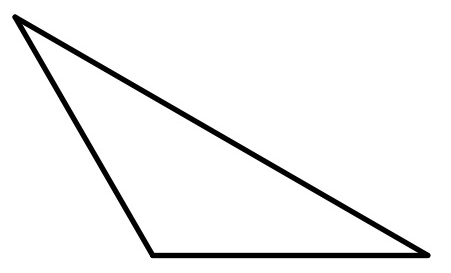
\includegraphics[width=3.6cm]{stats/2017/images/z_obtuse.png}
\end{center} \vspace{-0.7cm}

\itB Дан квадрат со стороной 1 см. Покажите, как разрезать его на остроугольные треугольники.

\itC Докажите, что сумма величин углов $A$ и $B$ на рисунке равна величине угла $C$.

\vspace{-0.4cm}
\begin{center}
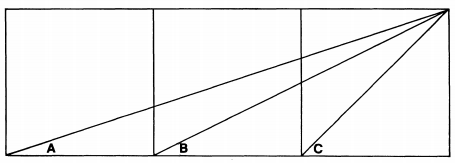
\includegraphics[width=8cm]{stats/2017/images/z_threesquares.png}
\end{center} \vspace{-0.4cm}
\end{itemize}